\documentclass{article}
\usepackage{amsfonts, amsmath, amssymb, amsthm} % Math notations imported
\usepackage{enumitem}
\usepackage[margin=1in]{geometry}
\usepackage{graphicx}
\graphicspath{{./images/}} % Path to images

\newtheorem{thm}{Theorem}
\newtheorem{prop}[thm]{Proposition}
\newtheorem{cor}[thm]{Corollary}

% title information
\title{Math 181A HW6}
\author{Neo Lee}
\date{05/09/2023}

% main content
\begin{document} 

% placing title information; comment out if using fancyhdr
\maketitle 

\textbf{Problem 14-1}
\begin{enumerate}[label={\alph*.}]
    \item 
    Let the null hypothesis be $H_0: p = 50\%$ and the alternative hypothesis be $H_1: p > 50\%$. Then the test statistic is
    \begin{align*}
        Z & = \frac{\hat{p} - p}{Var(p)}; \quad \hat{p} = \frac{548}{1053}; \quad Var(p) = \sqrt{\frac{p(1-p)}{n}} \\
        Z & = \frac{548/1053 - 0.5}{\sqrt{\frac{0.5(1-0.5)}{1053}}} \approx 1.325 < 1.96. \\
        \emph{p-value} & = P(Z > 1.325) \approx 0.0918 > 0.05.
    \end{align*}
    Hence, we failed to reject $H_0$. The data does not provide sufficient evidence to conclude that the majority of US adults favor passage.

    \item 
    \indent \\ 
    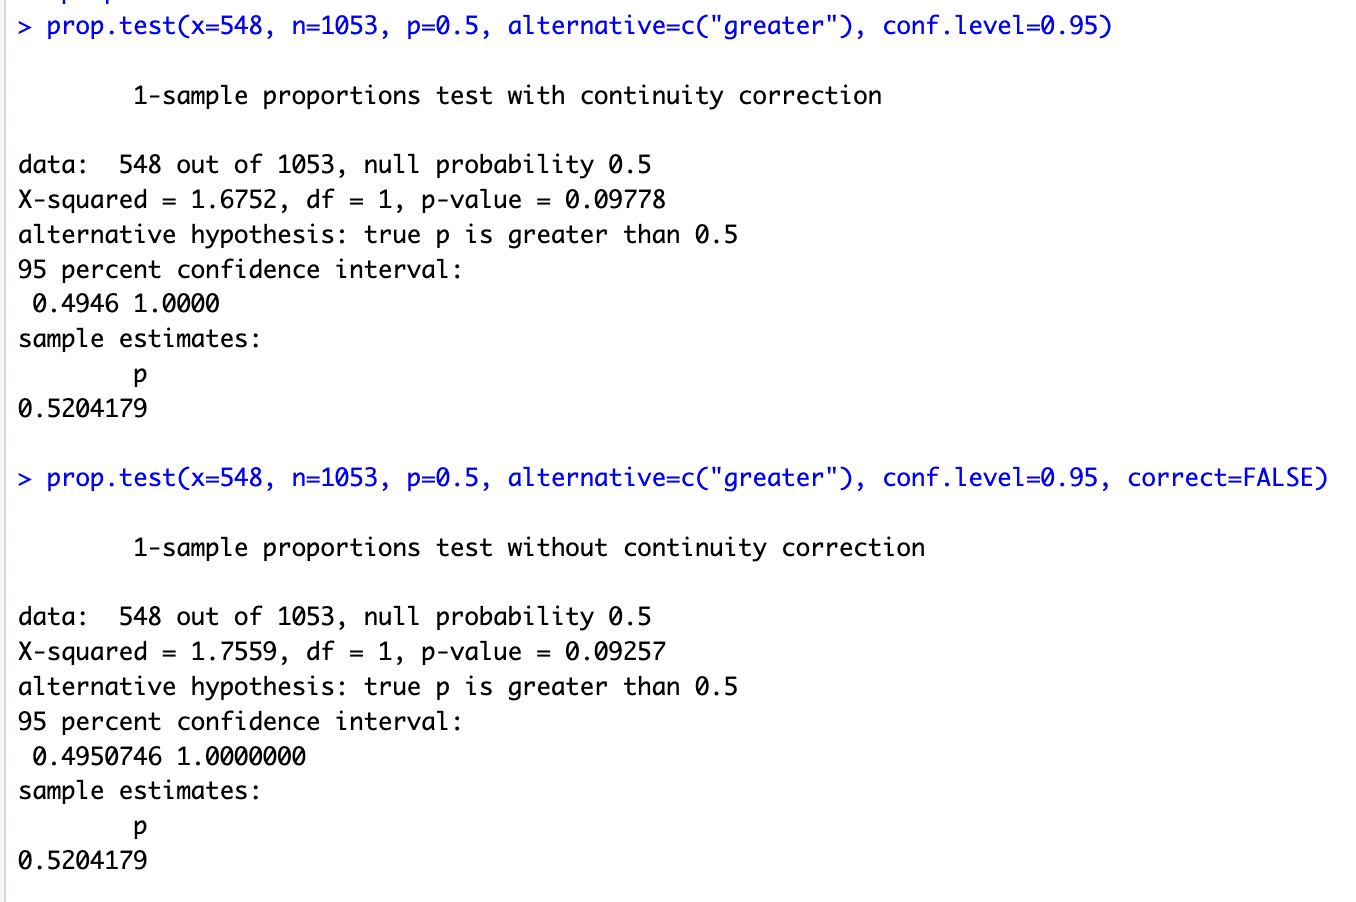
\includegraphics[scale=0.5]{prop.test}

    The hypothesis test with Yate's continuity correction yields a p-value of 0.09778, while the one without Yate's continuity correction yields a p-value of 0.0.09257. 
    They are similar to our calculation in part (a).
    Both p-values are greater than 0.05, so we failed to reject $H_0$. The data does not provide sufficient evidence to conclude that the majority of US adults favor passage.
\end{enumerate}

\end{document}